\documentclass{article}

\usepackage{graphicx}
\usepackage{indentfirst}
\usepackage[a4paper, total={6in, 8in}]{geometry}
\usepackage{hyperref}
\usepackage{fancyhdr}
\usepackage{xepersian}
\settextfont{B Nazanin}
\setlatintextfont{Times New Roman}

\begin{document}


%title page%
\begin{titlepage}
	\begin{center}
		\textbf{ \Huge{به نام خدا}}
	
		\vspace{0.2cm}
		
		
\includegraphics[width=0.4\textwidth]{sharif.png}\\
		\vspace{0.2cm}
		\textbf{ \Huge{آزمایش شماره ۱}}\\
		\vspace{0.25cm}
		\textbf{ \Large{آز معماری - دکتر سربازی آزاد}}
		\vspace{0.2cm}
		
		
		\large \textbf{دانشکده مهندسی کامپیوتر}\\\vspace{0.1cm}
		\large   دانشگاه صنعتی شریف\\\vspace{0.2cm}
		\large   ﻧﯿﻢ‌سال اول ۰۰-۰۱ \\\vspace{0.10cm}
		\large{گروه :}\\
		\large{\href{mailto:a.h.hadian@gmail.com}{امیرحسین هادیان - ۹۷۱۰۲۶۰۹}}\\
		\large{\href{mailto:mofayezi.m@gmail.com}{محمدرضا مفیضی - ۹۸۱۰۶۰۵۹}}\\
		\large{\href{mailto:a.hatam008@gmail.com}{علی حاتمی تاجیک - ۹۸۱۰۱۳۸۵}}\\
	\end{center}
\end{titlepage}
%title page%

\newpage

%pages header
\pagestyle{fancy}
\fancyhf{}
\fancyfoot{}
\setlength{\headheight}{59pt}
\cfoot{\thepage}
\lhead{آزمایش شماره ۱}
\rhead{
\includegraphics[width=0.1\textwidth]{sharif.png}\\
		دانشکده مهندسی کامپیوتر
}
\chead{آز معماری}
%pages header

\section{مقدمه}
در این سند گزارشی بر روند طراحی، پیاده‌سازی و تست یک مدار جمع کننده \lr{BCD} سه رقمی آورده ‌شده است. برای شبیه‌سازی این طراحی از نرم‌افزار \lr{Proteus} استفاده شده است.

\section{هدف}
هدف از انجام این آزمایش طراحی و ساخت یک جمع‌کننده ده‌دهی سه‌رقمی است. این جمع کننده ترکیبی خواهد بود و با تغییر ورودی‌ها تغییرات مستقیما در خروجی نمایان خواهند شد.

\section{طراحی}
طراحی این مدار به صورت \lr{Top-Down} صورت گرفته است. به همین‌ صورت نیز توضیح داده خواهد شد. در بالاترین لایه جمع‌کننده ده‌دهی سه بیتی ما به همراه کلید‌های ورودی و نمایشگر‌های \lr{7-Segments} قرار دارند که ورودی‌ها و نتیجه خروجی‌ را به ما نمایش می‌دهند. برای متصل کردن هر عدد ده‌رقمی از یک خط باس چهاربیتی استفاده شده است. از این خط باس در ماژول‌های پایین‌تر نیز برای تمیزی و سادگی نمایش بهره‌ برده شده است.
به ورودی
$ C_{in} $
 جمع‌کننده مقدار ثابت صفر وارد می‌شود. همینطور در در نمایش سه پایه نمایشگر به زمین متصل شده‌اند چرا که همواره صفر خواهند بود و تنها پایه اول که به
$C_{out}$
  متصل است (بزرگترین عددی که ممکن است تولید شود عدد 1999 خواهد بود). بالاترین سطح طراحی در شکل \ref{fig:final} آمده است.

\begin{figure}
	\centering
	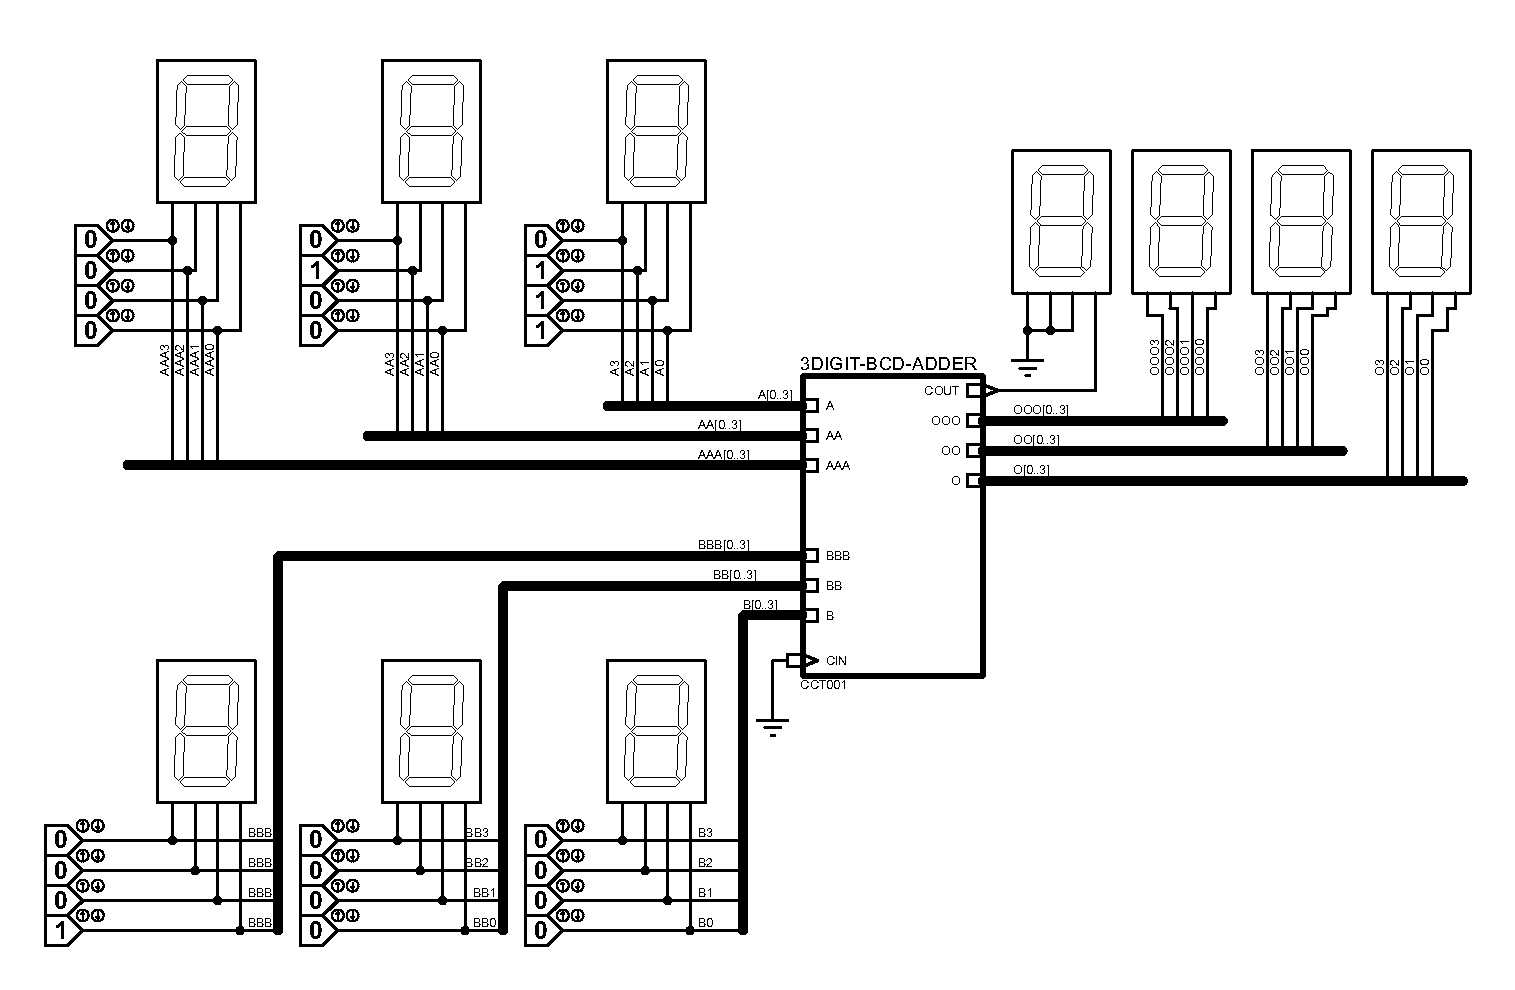
\includegraphics[scale=0.5]{./captures/final}
	\caption{مدار نهایی}
	\label{fig:final}
\end{figure}



\end{document}
